\documentclass[%
  reprint,
  superscriptaddress,
  showkeys,
  amsmath,amssymb,
  pra,
  longbibliography,
  floatfix
]{revtex4-2}

\usepackage[x11names]{xcolor}
\usepackage{graphicx}
\usepackage{tikz}
\usetikzlibrary{calc,intersections,shapes.geometric,positioning,
  arrows.meta,decorations.markings}
\usepackage{bm}
\usepackage{amsthm}          % required for definition/proposition/proof
\usepackage{orcidlink}
\usepackage{hyperref}         % load last

%--- theorem-like environments for revtex4-2 ---
\newtheorem{definition}{Definition}
\newtheorem{proposition}{Proposition}

\begin{document}

\title{A Geometric Theory of Contextual Semantic Capacity:\\
Concentration of Measure and Contextuality
in Large Language Models}

\author{Karl Svozil\,\orcidlink{0000-0001-6554-2802}}
\email{karl.svozil@tuwien.ac.at}
\affiliation{Institute for Theoretical Physics, TU Wien,
Wiedner Hauptstrasse 8-10/136, 1040 Vienna, Austria}

\date{\today}

\begin{abstract}
High-dimensional concentration geometry supplies the kinematic capacity for contextual semantic encoding in Large Language Models; hinge vectors and sense subspaces are one explicit geometric model of that capacity. Drawing on quantum contextuality, we analyze a polysemous token as a static hinge vector that gates the readout of meaning from a $(d-1)$-dimensional sense subspace orthogonal to it. L\'evy's lemma guarantees that exponentially many such subspaces can share a common hinge. We frame this as a geometric decomposition of contextual encoding, not a competing architecture, and propose probes for whether trained Transformers realize the structure.
\end{abstract}

\keywords{Large Language Models, Embeddings, Polysemy, Quantum
Contextuality, Concentration of Measure, L\'evy's Lemma, Contextual
Frames, Hinge Vectors, Superposition}

\maketitle

%===================================================================
\section{Introduction}
\label{sec:intro}
%===================================================================

Large Language Models (LLMs) operate on dense vector representations
of tokens in high-dimensional spaces.  The success of these systems
on linguistic tasks has been accompanied by a body of folk-theoretical
claims about how meaning is encoded geometrically: directions
correspond to features, distances to similarity, and arithmetic
operations on vectors to semantic analogies~\cite{mikolov2013}.  Yet
the mathematical underpinnings of these claims remain only partly
articulated.

This paper addresses one specific problem: \emph{polysemy}, the fact
that a single lexical item (e.g., ``bank'') can carry multiple,
mutually exclusive meanings depending on context.  In lexical
semantics, polysemy is distinguished from homonymy by the relatedness
of senses~\cite{pustejovsky1995}; for our purposes, the key feature
is that a single surface form must access distinct semantic content in
distinct contexts.  Modern Transformer-based LLMs handle this by
producing \emph{dynamic} contextual embeddings: the vector
representation of a token is iteratively transformed by self-attention
to absorb information from surrounding
tokens~\cite{Vaswani-2017-Attention}.  This approach is empirically
successful but conceptually opaque, since the same surface symbol is
mapped to different vectors depending on its sentential neighborhood.

We propose a geometric interpretation inspired by quantum
contextuality~\cite{specker-60,kochen1}.  On this reading, a
polysemous token can be analyzed as a single fixed unit
vector---a \emph{hinge vector}---that is shared as a common member of
multiple contextual frames.  The hinge vector itself does not change;
what changes is the contextual frame against which the surrounding
linguistic state is read out.  Crucially, the hinge vector plays an
operational role within the analysis: it \emph{gates} the readout by
setting its overall magnitude, while the specific sense is decoded
from the projection of the contextual hidden state onto the
hinge-perpendicular subspace.

We do not claim that this static formalism is a competing
\emph{architecture} to dynamic Transformer embeddings.  Rather, we
claim that any successful contextual encoding---static or
dynamic---must respect the geometric structure described here, and
that dynamic deformation in trained Transformers can be analyzed as
implicit realization of the same hinge-and-frame organization.  Layer
activations that move ``bank'' toward different regions of embedding
space in financial versus river contexts can be read as bringing a
particular sense subspace into alignment with downstream readout
heads.  The empirical question is then not which architecture is
correct, but whether trained models in fact organize their
representations in this way.  Section~\ref{sec:predictions} sets out
specific probes by which this can be tested.

The thesis of this paper is that \emph{high-dimensional
concentration-of-measure geometry provides the kinematic capacity
required for contextual semantic encoding}.  Contextuality supplies
the combinatorial architecture: a single hinge vector may be the
common element of multiple incompatible sense subspaces.  L\'evy's
lemma, applied to the linear overlap, supplies the geometric
mechanism: in high dimensions, almost all candidate sense directions
in the hinge-perpendicular subspace are nearly orthogonal to one
another, with deviations bounded by $2\exp(-cd\varepsilon^2)$.
Together, these imply that exponentially many approximately
independent sense subspaces can share a common hinge vector.  The Johnson--Lindenstrauss lemma~\cite{johnson-1984}, often invoked
in similar contexts, arises from the same concentration phenomenon.

The analysis is conceptually adjacent to the \emph{superposition
hypothesis} in mechanistic
interpretability~\cite{elhage2022superposition}, which holds that
neural networks pack many features into nearly-orthogonal directions
in a low-dimensional space, with the count bounded by exactly the
kind of concentration estimate we use.  The present formalism differs
in identifying a specific structural pattern---hinge-and-frame rather
than unstructured overcomplete dictionary---and in foregrounding the
gating role of the hinge vector.  In a sparse-coding picture,
polysemous tokens correspond to special \emph{junction} directions
where multiple feature subspaces intersect.

The paper is organized as follows.
Section~\ref{sec:geometry} develops the geometric foundations:
quasi-orthogonality, L\'evy's lemma on the linear overlap, the
relation to Johnson--Lindenstrauss, and the definition of stable
contextual frames.
Section~\ref{sec:polysemy} introduces hinge vectors, the
gated-subspace readout of context states, the bridge between
concentration and contextuality, a proposition counting
distinguishable sense subspaces sharing a hinge vector, and the
relation to dynamic Transformer embeddings.
Section~\ref{sec:attention} discusses self-attention as approximate
frame readout, formulates frame selection as a latent-variable
model, and analyzes the role of stochastic decoding.
Section~\ref{sec:discussion} addresses the relation to the
superposition hypothesis, limitations including the anisotropy
threat, empirical predictions, and the scope of the quantum analogy.

\medskip
\noindent\textbf{Notation.}
Throughout, $\mathbb{R}^d$ denotes Euclidean $d$-space with the
standard inner product $\bm{u}^\intercal\bm{v}$ and induced norm
$\|\bm{v}\|=\sqrt{\bm{v}^\intercal\bm{v}}$;
$S^{d-1}=\{\bm{v}\in\mathbb{R}^d:\|\bm{v}\|=1\}$ is the unit sphere;
$\bm{I}$ is the identity matrix; $(\cdot)^\intercal$ denotes
transpose; $\|\cdot\|_{\mathrm{op}}$ is the operator (spectral) norm;
$A\succeq 0$ means $A$ is positive semi-definite; $\mathbb{P}$ and
$\mathbb{E}$ denote probability and expectation under the uniform
(Haar) measure on $S^{d-1}$ unless otherwise noted; $O(\cdot)$ and
$\Omega(\cdot)$ are the standard Landau symbols.  We write
$\mathrm{ReLU}(x)=\max(0,x)$ and use $\sigma$ for the logistic
sigmoid $\sigma(x)=(1+e^{-x})^{-1}$.  Universal positive constants
are denoted $c$, $c'$, possibly differing between occurrences.

%===================================================================
\section{Concentration Geometry and Frame Capacity}
\label{sec:geometry}
%===================================================================

\subsection{Quasi-Orthogonality}
\label{sec:quasi}

Let $\bm{v}_1,\dots,\bm{v}_N \in \mathbb{R}^d$ be unit vectors.
The vectors are \emph{strictly orthogonal} if
$\bm{v}_i^\intercal \bm{v}_j = 0$ for all $i \neq j$.  By
elementary linear algebra, at most $N=d$ such vectors can coexist in
$\mathbb{R}^d$.

This linear bound is restrictive.  Many semantic features that one
might wish to encode as directions need not be perfectly
distinguishable; it suffices that they be \emph{nearly}
distinguishable.  We therefore introduce
$\varepsilon$-quasi-orthogonality: a set of unit vectors is
$\varepsilon$-quasi-orthogonal if
\begin{equation}
    |\bm{v}_i^\intercal \bm{v}_j| \le \varepsilon,
    \qquad i \neq j.
    \label{eq:quasi}
\end{equation}
Since exact orthogonality is neither achievable nor necessary in
realistic embedding spaces, quasi-orthogonality is the operationally
meaningful notion throughout this paper.

\subsection{L\'evy's Lemma on the Linear Overlap}
\label{sec:levy}

The exponential capacity of high-dimensional spaces for
quasi-orthogonal vectors is closely related to
concentration-of-measure phenomena.  In high dimensions, most of the
volume of the unit sphere $S^{d-1}$ lies near the equator relative to
any fixed direction.  Consequently, two independently sampled random
unit vectors are almost orthogonal with overwhelming probability.

This may be formalized using L\'evy's
lemma~\cite{ledoux2001concentration,milman1986asymptotic}.  Let
$f\colon S^{d-1}\to\mathbb{R}$ be an $L$-Lipschitz function, i.e.,
$|f(\bm{x})-f(\bm{y})|\le L\|\bm{x}-\bm{y}\|$ for all
$\bm{x},\bm{y}\in S^{d-1}$.  Then for any $\delta>0$,
\begin{equation}
    \mathbb{P}\!\left(\left|f(\bm{v})-\mathbb{E}[f]\right|
    \ge\delta\right)
    \le 2\exp\!\left(-\frac{c\,d\,\delta^2}{L^2}\right),
    \label{eq:levy-general}
\end{equation}
where $c>0$ is a universal constant and the probability is taken over
the uniform measure on $S^{d-1}$.

To obtain quasi-orthogonality, we apply L\'evy's lemma to the
\emph{linear} overlap
$f_{\bm{u}}(\bm{v}) = \bm{u}^\intercal\bm{v}$, which is
$1$-Lipschitz by the Cauchy--Schwarz inequality.  By symmetry,
$\mathbb{E}[f_{\bm{u}}]=0$.  Therefore, for any $\varepsilon>0$,
\begin{equation}
    \mathbb{P}\!\left(|\bm{u}^\intercal\bm{v}|
    \ge \varepsilon\right)
    \le 2\exp(-c\,d\,\varepsilon^2).
    \label{eq:linear-levy}
\end{equation}
For the standard normalized surface measure on $S^{d-1}$, an explicit
form of the constant gives
$2\exp(-(d-1)\varepsilon^2/2)$~\cite{ledoux2001concentration}.  Two
independent random unit vectors are therefore
$\varepsilon$-quasi-orthogonal with probability at least
$1-2\exp(-cd\varepsilon^2)$, and typical overlap amplitudes scale as
$d^{-1/2}$.

The geometric significance is immediate: in sufficiently high
dimension, almost all directions are nearly orthogonal to any given
direction, and this quasi-orthogonality is a robust, generic property
of high-dimensional spheres.

\subsection{Relation to the Johnson--Lindenstrauss Lemma}
\label{sec:jl}

The concentration phenomenon underlying
Eq.~\eqref{eq:linear-levy} is closely related to the
Johnson--Lindenstrauss (JL) lemma~\cite{johnson-1984}, which states
that any set of $n$ points in Euclidean space can be projected into a
space of dimension $k = O(\varepsilon^{-2}\log n)$ while preserving
all pairwise distances to within a factor of $(1\pm\varepsilon)$.

Conceptually, both results arise from the same high-dimensional
geometric fact: random projections and random directions are highly
regular in large dimension.  The JL lemma emphasizes the stability of
finite metric structure under random projection, whereas L\'evy's
lemma emphasizes the concentration of Lipschitz observables around
their mean values on high-dimensional spheres.  The two are
mathematically intertwined---one can derive the JL lemma from
concentration of measure on the sphere applied to projection
norms~\cite{Dasgupta-2003}---but they highlight complementary
aspects of the same phenomenon.

For the present purposes, L\'evy's lemma is the more natural tool,
because the relevant issue is not dimensionality reduction of a finite
dataset, but the typical quasi-orthogonality and abundance of semantic
directions in high-dimensional embedding spaces.

\subsection{Stable Contextual Frames}
\label{sec:stable}

A contextual frame is not merely a collection of pairwise
quasi-orthogonal vectors.  Pairwise bounds such as
$|\bm{e}_i^\intercal\bm{e}_j|\le\varepsilon$ do not guarantee a
well-conditioned frame when $d$ is large, because the cumulative
spectral effect of many small off-diagonal entries can be significant.
By the Gershgorin circle theorem, pairwise quasi-orthogonality only
implies
$\|\bm{G}-\bm{I}\|_{\mathrm{op}}\le (d-1)\varepsilon$, which is
uninformative for $\varepsilon=O(1)$ and $d\sim 10^3$.  We therefore
require a stronger condition.

\begin{definition}[$\rho$-stable contextual frame]
\label{def:stable}
A contextual frame
$\mathcal{F}^{\mathcal{C}}
=\{\bm{e}_1^{\mathcal{C}},\ldots,\bm{e}_d^{\mathcal{C}}\}$
with frame matrix
$\bm{F}^{\mathcal{C}}
=[\bm{e}_1^{\mathcal{C}}\;\cdots\;\bm{e}_d^{\mathcal{C}}]$
is called \emph{$\rho$-stable} if its Gram matrix
$\bm{G}^{\mathcal{C}}
=(\bm{F}^{\mathcal{C}})^\intercal\bm{F}^{\mathcal{C}}$
satisfies
\begin{equation}
    \|\bm{G}^{\mathcal{C}}-\bm{I}\|_{\mathrm{op}}
    \le \rho <1.
    \label{eq:stable-frame}
\end{equation}
Exact orthonormal bases correspond to $\rho=0$.
\end{definition}

Stability ensures that all singular values of
$\bm{F}^{\mathcal{C}}$ lie between $\sqrt{1-\rho}$ and
$\sqrt{1+\rho}$.  Consequently, the dual frame
$\widetilde{\bm{F}}^{\mathcal{C}}
= \bm{F}^{\mathcal{C}}(\bm{G}^{\mathcal{C}})^{-1}$
is well-defined and satisfies
$\|\widetilde{\bm{F}}^{\mathcal{C}}\|_{\mathrm{op}}
\le (1-\rho)^{-1/2}$.
The dual-frame readout is therefore numerically stable.

\subsection{Exponential Packing}
\label{sec:packing}

The concentration bound~\eqref{eq:linear-levy} yields an exponential
packing result for individual vectors.  Sample $N$ unit vectors
independently and uniformly from $S^{d-1}$.  By a union bound over
the $\binom{N}{2}<N^2/2$ pairs,
\begin{equation}
    \mathbb{P}\!\left(\exists\, i\ne j\colon
    |\bm{v}_i^\intercal\bm{v}_j| \ge \varepsilon\right)
    < N^2\exp(-c\,d\,\varepsilon^2).
    \label{eq:union}
\end{equation}
This probability is less than one---and hence an
$\varepsilon$-quasi-orthogonal family of size $N$ exists---provided
\begin{equation}
    N < \exp\!\left(\tfrac{c}{2}\,d\,\varepsilon^2\right).
    \label{eq:packing}
\end{equation}

For typical LLM embedding dimensions ($d \sim 10^3$ to $10^4$) and
modest tolerances ($\varepsilon \sim 0.1$), this bound permits
enormous numbers of quasi-orthogonal directions.  We refer to this
exponentially large supply as the \emph{quasi-dimensionality} of the
embedding space.

We emphasize, however, that the packing bound controls only pairwise
overlaps.  As the Gershgorin remark above shows, pairwise control does
not by itself yield operator-norm control over a frame matrix.  The
frame-level analogue requires a separate construction, which we
present below in Proposition~\ref{prop:frames}.

%===================================================================
\section{Hinge Vectors and Sense Subspaces}
\label{sec:polysemy}
%===================================================================

\subsection{The Hinge-Vector Formalism}
\label{sec:hinge}

We propose the following formalism.  Each token $t$ is assigned a
fixed unit vector $\bm{v}(t) \in \mathbb{R}^d$, called its
\emph{hinge vector}.  Each \emph{context} $\mathcal{C}$ in which $t$
appears is represented by a $\rho$-stable contextual frame
$\mathcal{F}^{\mathcal{C}}
= \{\bm{e}_1^{\mathcal{C}}, \dots, \bm{e}_d^{\mathcal{C}}\}$
with frame matrix $\bm{F}^{\mathcal{C}}$, organized so that
\begin{equation}
    \bm{e}_1^{\mathcal{C}} = \bm{v}(t).
    \label{eq:hinge}
\end{equation}
The remaining frame vectors $\{\bm{e}_2^{\mathcal{C}},\dots,
\bm{e}_d^{\mathcal{C}}\}$ are unit vectors in
$\bm{v}(t)^\perp\subset\mathbb{R}^d$ and span a
$(d{-}1)$-dimensional \emph{sense subspace}
\begin{equation}
    \mathcal{S}^{\mathcal{C}}
    = \mathrm{span}\{\bm{e}_2^{\mathcal{C}},
                     \dots,\bm{e}_d^{\mathcal{C}}\}
    \subset \bm{v}(t)^\perp.
    \label{eq:sense-subspace}
\end{equation}
A token is \emph{polysemous} if its hinge vector belongs in this way
to two or more contextual frames, each carrying a distinct sense
subspace.  For example, $\bm{v}(\text{bank})$ might serve as the
hinge of a finance frame, a river frame, and a tilt-of-aircraft frame,
each with its own sense subspace inside
$\bm{v}(\text{bank})^\perp$.

\medskip
\noindent\textbf{The gated-subspace readout of context.}
The meaning of a polysemous token is not contained in its hinge
vector alone, because in every frame that contains it, the hinge has
the same coordinates: $(1,0,\dots,0)$.  Meaning is relational.  It
emerges from the interaction between the hinge vector and the
surrounding linguistic context, mediated by the sense subspace.

Given an input context $x$, let
$\bm{h}(x)\in\mathbb{R}^d$ denote the contextual state---in a static
model, a vector derived from the surrounding tokens; in a trained
model, the hidden state produced by preceding layers.  We decompose
$\bm{h}(x)$ along the hinge:
\begin{equation}
    \bm{h}(x)
    = h_\parallel(x)\,\bm{v}(t) + \bm{h}_\perp(x),
    \qquad
    h_\parallel(x)
    = \bm{v}(t)^\intercal\bm{h}(x),
    \label{eq:hinge-decomp}
\end{equation}
with $\bm{h}_\perp(x)\in\bm{v}(t)^\perp$.  The two components play
distinct roles: $h_\parallel(x)$ measures how strongly the context
\emph{engages} the token at all, while $\bm{h}_\perp(x)$ carries the
\emph{sense-disambiguating} information.

The dual-frame readout in frame $\mathcal{C}$ is performed within the
sense subspace.  Let
$\bm{F}^{\mathcal{C}}_{\mathcal{S}}
=[\bm{e}_2^{\mathcal{C}}\;\cdots\;\bm{e}_d^{\mathcal{C}}]$ be the
frame matrix restricted to the sense subspace, and let
$\widetilde{\bm{F}}^{\mathcal{C}}_{\mathcal{S}}$ denote its dual.
Then
\begin{equation}
    \bm{\alpha}^{\mathcal{C}}(x)
    = \bigl(\widetilde{\bm{F}}^{\mathcal{C}}_{\mathcal{S}}
      \bigr)^\intercal\,\bm{h}_\perp(x)
    \in \mathbb{R}^{d-1}
    \label{eq:context-readout}
\end{equation}
gives the dual-frame coefficients of $\bm{h}_\perp(x)$ in
$\mathcal{S}^{\mathcal{C}}$.

The \emph{sense score} of frame $\mathcal{C}$ for context $x$ is
\begin{equation}
    s_{\mathcal{C}}(x)
    = h_\parallel(x)^2
      \cdot r_{\mathcal{C}}\bigl(\bm{h}_\perp(x)\bigr),
    \label{eq:sense-score}
\end{equation}
where $r_{\mathcal{C}}\colon\bm{v}(t)^\perp\to\mathbb{R}_{\ge 0}$ is
a within-subspace selector: it scores how well the sense subspace
$\mathcal{S}^{\mathcal{C}}$ aligns with $\bm{h}_\perp(x)$.  Three
natural choices for $r_{\mathcal{C}}$ are
\begin{enumerate}
\item the squared norm of the dual-frame expansion,
$r_{\mathcal{C}} = \|\bm{\alpha}^{\mathcal{C}}(x)\|^2$, when the
frame is characterized purely by its orientation;
\item the squared overlap with a designated direction
$\bm{w}^{\mathcal{C}}\in\mathcal{S}^{\mathcal{C}}$,
$r_{\mathcal{C}} = (\bm{w}^{\mathcal{C}\,\intercal}
\bm{h}_\perp(x))^2$, when a single sense-distinguishing axis is
appropriate; or
\item a learned positive functional, e.g.\ a quadratic form
$\bm{h}_\perp(x)^\intercal A^{\mathcal{C}}\bm{h}_\perp(x)$ with
$A^{\mathcal{C}}\succeq 0$, when training infers the relevant
within-subspace structure.
\end{enumerate}
The selected frame is
\begin{equation}
    \mathcal{C}^*(x)
    = \arg\max_{\mathcal{C}}\, s_{\mathcal{C}}(x).
    \label{eq:frame-selection}
\end{equation}
The meaning of token $t$ in context $x$ is the relational triple
\begin{equation}
    \bigl(\bm{v}(t),\;\mathcal{C}^*(x),\;
    \bm{\alpha}^{\mathcal{C}^*(x)}(x)\bigr).
    \label{eq:meaning}
\end{equation}

\medskip
\noindent\textbf{On the form of the gating prefactor.}
The choice $h_\parallel(x)^2$ in Eq.~\eqref{eq:sense-score} is a
representative member of a family of admissible gating functions
$g(h_\parallel)\colon\mathbb{R}\to\mathbb{R}_{\ge 0}$, all sharing
two essential properties: (i)~$g(0)=0$, so that hidden states
orthogonal to the hinge produce no readout, and (ii)~$g$ is
non-decreasing in $|h_\parallel|$, so that stronger engagement with
the hinge amplifies the score.  Natural alternatives include
$|h_\parallel|$, $\mathrm{ReLU}(h_\parallel)$ (sign-sensitive,
firing only on positive overlap), and learned smooth gates
$\sigma(\beta h_\parallel)$.  Squaring is the simplest scalar that is
smooth, non-negative, and zero only at $h_\parallel=0$, which
motivates it as a default; it does, however, discard the sign of
$h_\parallel$, which may itself carry information (e.g., in
antonymic contexts).  In a learning setting, $g$ would naturally be
inferred from data alongside the frames.

The multiplicative form $g(h_\parallel)\cdot
r_{\mathcal{C}}(\bm{h}_\perp)$ is also a choice, distinguishable
from additive alternatives such as $|h_\parallel|+r_{\mathcal{C}}$.
Multiplicative gating expresses the conjunction ``the token is
engaged \emph{and} this sense is the one that fits,'' and ensures
that no sense scores positively when engagement is absent; additive
forms do not have this property.  We emphasize that the
multiplicative form does not assume statistical independence between
$h_\parallel$ and $\bm{h}_\perp$ in any context distribution---it
specifies a functional combination, not a factorization of a joint
density.  The form of the gating function and the shape of
$r_{\mathcal{C}}$ are independently choosable; the role of the
formalism is to constrain their product to vanish when the hinge is
not engaged.\footnote{For ease of exposition we treat the set of
contextual frames as discrete, indexed by sense.  In a learning
setting, frames could equally be parameterized continuously---e.g.,
as elements of the Stiefel manifold $V_{d-1}(\mathbb{R}^d)$---in
which case Eqs.~\eqref{eq:sense-score}--\eqref{eq:frame-selection}
become a continuous optimization rather than a discrete argmax.  The
discrete formulation is natural for sense disambiguation, where
senses are categorical in lexicography, and we use it throughout.}

\medskip
\noindent\textbf{Why the hinge vector matters.}  In this formalism,
the hinge $\bm{v}(t)$ plays a genuinely operational role: through
the prefactor $g(h_\parallel(x))$, it gates the entire readout.
When the contextual state is orthogonal to $\bm{v}(t)$, no frame
associated with $t$ scores positively, and the token is not engaged
by the context.  When $h_\parallel(x)$ is large, the readout is
amplified and the within-subspace selector $r_{\mathcal{C}}$ decides
which sense applies.  Different hinges (for different tokens) induce
different decompositions $\bm{h} = h_\parallel \bm{v} +
\bm{h}_\perp$, and hence different sense subspaces in
$\bm{v}(t)^\perp$.  The geometry of the hinge is therefore not mere
bookkeeping: it is what determines which subspace of context is
exposed for sense disambiguation.

\subsection{Concentration as the Geometric Substrate
of Contextuality}
\label{sec:bridge}

Quantum contextuality concerns the coexistence of multiple
incompatible measurement bases sharing common
vectors~\cite{specker-60,kochen1,Gleason}.  In the present setting,
the analogous structure is a family of semantic contexts represented
by distinct contextual frames that partially overlap through a shared
hinge.

The central geometric question is whether sufficiently many nearly
independent sense subspaces can coexist in
$\bm{v}(t)^\perp \cong \mathbb{R}^{d-1}$ without destructive
interference.  This question has a sharp answer:

\begin{enumerate}
\item \emph{Contextuality} provides the combinatorial
architecture---the logical possibility that a single hinge vector
simultaneously belongs to multiple incompatible frames, each
defining a distinct sense subspace.
\item \emph{Concentration of measure} provides the geometric
capacity---the guarantee that in high dimensions, exponentially many
such subspaces can coexist with only weak mutual interference.
\end{enumerate}

By L\'evy's lemma applied within $\bm{v}(t)^\perp$, once the hinge
vector is fixed, the overwhelming majority of candidate sense
directions remain quasi-orthogonal to one another.  A single hinge
may therefore simultaneously support a large number of approximately
independent sense subspaces.  Concentration of measure supplies the
geometric substrate that makes contextual encoding scalable.

The role played by concentration here is analogous to the role played
by large Hilbert-space dimension in quantum contextuality
constructions: the combinatorial richness of intertwining contexts
becomes increasingly abundant as dimension grows.  The present
proposal differs, however, in two important respects.  First, exact
orthogonality is replaced by quasi-orthogonality, which is both
geometrically typical and operationally sufficient for semantic
disambiguation.  Second, quantum contextuality carries physical
content beyond geometry: the Kochen--Specker theorem~\cite{kochen1}
proves that no noncontextual hidden-variable model can reproduce
quantum predictions, regardless of the dimension.  In our semantic
setting, no analogous no-go theorem has been established.  The
contextuality we invoke is structural---it concerns the combinatorial
pattern of frame-sharing---rather than foundational in the sense of
constraining hidden-variable theories.

\subsection{Many Sense Subspaces Sharing One Hinge Vector}
\label{sec:counting}

The packing bound~\eqref{eq:packing} counts individual
quasi-orthogonal vectors.  The central claim of this paper, however,
concerns sense \emph{subspaces}---structured $(d{-}1)$-dimensional
complements of a fixed hinge---that share a common hinge vector.  The
following proposition shows that exponentially many such subspaces
exist with controlled mutual coherence.

\begin{proposition}[Sense-subspace capacity]
\label{prop:frames}
Fix a unit vector $\bm{v}_0\in S^{d-1}$.  For any fixed
$\varepsilon>0$ and sufficiently large $d$, there exist
\begin{equation}
    M \ge \frac{1}{d-1}\exp(c'\varepsilon^2 (d-1))
    \label{eq:frame-count}
\end{equation}
orthonormal contextual frames
$\mathcal{C}_1,\ldots,\mathcal{C}_M$ such that each frame contains
$\bm{v}_0$ as its first vector and, for any two distinct frames
$\mathcal{C}_a\neq \mathcal{C}_b$,
\begin{equation}
    \left|(\bm{e}_i^{\mathcal{C}_a})^\intercal
    \bm{e}_j^{\mathcal{C}_b}\right| \le \varepsilon
    \label{eq:cross-frame}
\end{equation}
for all non-shared frame vectors $i,j\ge 2$, with a universal
constant $c'>0$.
\end{proposition}

\begin{proof}
The orthogonal complement $\bm{v}_0^\perp$ has dimension $d-1$.
Sample $M$ independent Haar-random orthonormal bases of
$\bm{v}_0^\perp$ and prepend $\bm{v}_0$ to each, yielding $M$
orthonormal frames of $\mathbb{R}^d$ with shared first vector
$\bm{v}_0$.

For any fixed vector $\bm{e}_i^{\mathcal{C}_a}\in\bm{v}_0^\perp$
(with $i\ge 2$), the marginal distribution of any single basis vector
$\bm{e}_j^{\mathcal{C}_b}$ ($j\ge 2$) drawn from an independent
Haar-random orthonormal basis of $\bm{v}_0^\perp$ is uniform on the
unit sphere of $\bm{v}_0^\perp$.  By L\'evy's lemma applied within
this $(d-1)$-dimensional sphere,
\begin{equation}
    \mathbb{P}\!\left(\left|(\bm{e}_i^{\mathcal{C}_a})^\intercal
    \bm{e}_j^{\mathcal{C}_b}\right| \ge \varepsilon\right)
    \le 2\exp\bigl(-c(d-1)\varepsilon^2\bigr).
    \label{eq:cross-tail}
\end{equation}
Within-frame correlations do not enter because the bound concerns
only \emph{cross}-frame pairs.  There are at most $M^2(d-1)^2$ such
pairs.  By the union bound, all cross-frame overlaps satisfy
$\le\varepsilon$ with positive probability provided
\begin{equation}
    M^2(d-1)^2\cdot 2\exp(-c(d-1)\varepsilon^2) < 1.
\end{equation}
This is satisfied for
$M = \lfloor (d-1)^{-1}\exp(c'\varepsilon^2 (d-1))\rfloor$ with a
suitable universal constant $c'>0$.
\end{proof}

For typical LLM dimensions ($d \sim 10^3$) and tolerances
($\varepsilon \sim 0.1$), Proposition~\ref{prop:frames} implies that
the number of available sense subspaces sharing a single hinge
vector is exponentially large, far exceeding the number of distinct
senses that any natural-language token carries.

The proposition as stated produces frames with $\rho=0$ (exact
orthonormality).  A relaxed version permitting $\rho$-stable but
non-orthonormal frames could be obtained by sampling near-orthonormal
frames---e.g., perturbations of Haar-random bases or outputs of a
soft-stability regularizer---and applying the same union-bound
argument together with a stability bound.  We do not pursue this
extension here; the orthonormal case suffices to establish the
capacity claim.

\subsection{Intertwining Contextual Frames}
\label{sec:intertwine}

Two distinct contextual frames that share at least one common vector
are called \emph{intertwined}.  Figure~\ref{fig:intertwining}
illustrates a simple case: three contextual frames sharing a single
hinge vector $\bm{v}(\text{bank})$, each carrying a distinct sense
subspace within $\bm{v}(\text{bank})^\perp$.  For visualization, a
single distinguishing direction within each sense subspace is shown.

\begin{figure}[t]
\centering
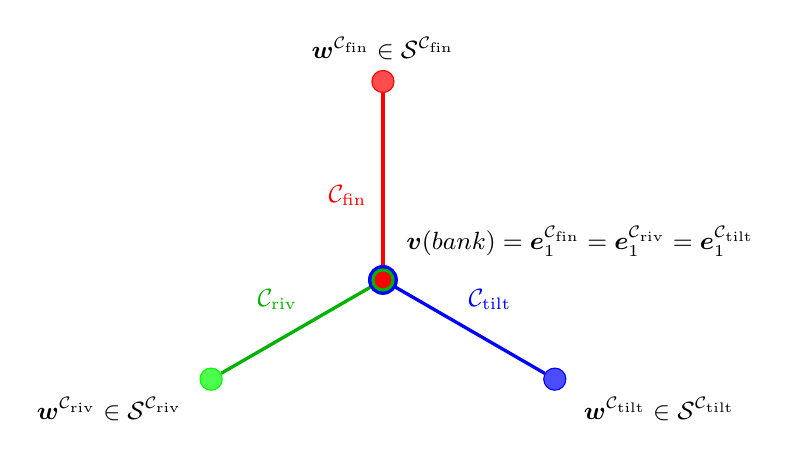
\begin{tikzpicture}[scale=0.6,
    outer/.style={circle, draw, minimum size=8pt,
                  inner sep=0pt, font=\footnotesize},
    lab/.style={font=\small}]
% central shared vector
\coordinate (c) at (0,0);

\node[lab, above right=7pt] at (c)
{$\bm{v}(\text{bank})
=\bm{e}_1^{\mathcal{C}_{\rm fin}}
=\bm{e}_1^{\mathcal{C}_{\rm riv}}
=\bm{e}_1^{\mathcal{C}_{\rm tilt}}$};

% outer distinguishing vectors
\node[outer, red, fill=red!70,
      label={[lab]above:
      $\bm{w}^{\mathcal{C}_{\rm fin}}
      \in\mathcal{S}^{\mathcal{C}_{\rm fin}}$}]
      (fin) at (90:4.2cm) {};

\node[outer, green, fill=green!70,
      label={[lab, xshift=-4pt]below left:
      $\bm{w}^{\mathcal{C}_{\rm riv}}
      \in\mathcal{S}^{\mathcal{C}_{\rm riv}}$}]
      (riv) at (210:4.2cm) {};

\node[outer, blue, fill=blue!70,
      label={[lab, xshift=4pt]below right:
      $\bm{w}^{\mathcal{C}_{\rm tilt}}
      \in\mathcal{S}^{\mathcal{C}_{\rm tilt}}$}]
      (tilt) at (330:4.2cm) {};

% edges labelled by contextual frames
\draw[very thick, red] (c) --
      node[lab, left=2pt, pos=0.45]
      {$\mathcal{C}_{\rm fin}$} (fin);

\draw[very thick, green!70!black] (c) --
      node[lab, above left=1pt, pos=0.45]
      {$\mathcal{C}_{\rm riv}$} (riv);

\draw[very thick, blue] (c) --
      node[lab, above right=1pt, pos=0.45]
      {$\mathcal{C}_{\rm tilt}$} (tilt);

% central concentric disks
\filldraw[blue, very thick] (c) circle (8pt);
\filldraw[green!70!black, very thick] (c) circle (6pt);
\filldraw[red, very thick] (c) circle (4pt);
\end{tikzpicture}
\caption{%
Three intertwined contextual frames
$\mathcal{C}_{\rm fin}$, $\mathcal{C}_{\rm riv}$, and
$\mathcal{C}_{\rm tilt}$ sharing the common hinge vector
$\bm{v}(\text{bank})$ (financial institution, riverside, and
aircraft-tilt senses).  In each frame, the hinge is the first frame
vector, $\bm{e}_1^{\mathcal{C}}=\bm{v}(\text{bank})$.  Each frame
carries a $(d{-}1)$-dimensional sense subspace
$\mathcal{S}^{\mathcal{C}}\subset\bm{v}(\text{bank})^\perp$.
For visualization, a single distinguishing direction
$\bm{w}^{\mathcal{C}}\in\mathcal{S}^{\mathcal{C}}$ within each
sense subspace is shown.  The semantic interpretation is not
contained in $\bm{v}(\text{bank})$ alone, but in the gated readout
of the surrounding context state through the
hinge-perpendicular component~\eqref{eq:context-readout}.%
}
\label{fig:intertwining}
\end{figure}

\subsection{Relation to Dynamic Contextual Embeddings}
\label{sec:comparison}

Standard Transformer-based LLMs handle polysemy through dynamic
embeddings.  The token ``bank'' is initially mapped to a single
static embedding $\bm{v}_0(\text{bank})$, but this vector is then
transformed layer by layer through self-attention into a
context-dependent vector $\bm{v}_L(\text{bank} \mid \text{context})$
that depends explicitly on the surrounding tokens.

The hinge-and-frame analysis is not in opposition to this picture.
It offers a structural decomposition under which the dynamic
trajectory $\bm{v}_0\to\bm{v}_L$ can be read as implicitly performing
frame selection: layer activations move the representation so as to
bring a particular sense subspace into alignment with downstream
readout heads.  The static embedding plays the role of a candidate
hinge; the layer-induced offset corresponds to the
hinge-perpendicular component $\bm{h}_\perp(x)$; and the geometry of
nearly-orthogonal sense subspaces explains why distinct senses can
be cleanly separated by the network's downstream computations.
Table~\ref{tab:comparison} summarizes how the two descriptions
correspond.

\begin{table}[t]
\caption{Two descriptions of the same contextual phenomenon.  The
hinge-and-frame analysis is presented as a static decomposition of
what dynamic Transformers do, not as a competing architecture.}
\label{tab:comparison}
\begin{ruledtabular}
\begin{tabular}{lcc}
 & \textbf{Dynamic description} & \textbf{Static decomposition} \\
\hline
Token vector & Changes per context & Fixed (hinge) \\
Context carrier & Layer activations & Hinge-perpendicular state \\
Polysemy mechanism & Vector deformation & Gated subspace readout \\
Geometric resource & Network depth & Quasi-dimensionality \\
Readout & Final-layer projection & Dual-frame coefficients \\
\end{tabular}
\end{ruledtabular}
\end{table}

What would distinguish the two descriptions empirically?  The
hinge-and-frame analysis predicts that for a polysemous token, the
projection of contextual hidden states onto the orthogonal
complement of the static input embedding---i.e., the candidate
hinge---should partition cleanly by sense.  A purely dynamic account,
by contrast, would not single out the static input embedding as a
preferred direction; deformation could in principle proceed in any
direction without privileging the original embedding.  The
prediction is therefore not about which architecture is correct, but
about whether trained models exhibit hinge-anchored organization.
Section~\ref{sec:predictions} formulates concrete probes for this
question.


%===================================================================
\section{Attention, Latent Frames, and Stochastic Decoding}
\label{sec:attention}
%===================================================================

\subsection{Self-Attention as Approximate Frame Selection}
\label{sec:attn-frames}

The static contextual encoding of Section~\ref{sec:polysemy} is
conceptually different from the dynamic embeddings of Transformers,
but the two are not unrelated.  Self-attention computes, for each
token position, a convex combination of value vectors weighted by
attention scores:
\begin{equation}
    \bm{h}' = \sum_{j} \alpha_j \,\bm{v}_j,
    \qquad
    \alpha_j
    = \frac{\exp(\bm{q}^\intercal \bm{k}_j / \sqrt{d})}
           {\sum_{j'}\exp(\bm{q}^\intercal \bm{k}_{j'} / \sqrt{d})},
    \label{eq:attention}
\end{equation}
where $\bm{q}$, $\bm{k}_j$, and $\bm{v}_j$ are the query, key, and
value vectors of standard self-attention, and $\bm{h}'$ is the
attention output.

If the keys $\{\bm{k}_j\}$ are interpreted as frame vectors and the
values as semantic content vectors, then the attention output is a
weighted sum of frame elements.  Any $\rho$-stable frame admits a
dual-frame readout (Section~\ref{sec:stable}); the tight-frame
condition $\sum_j \bm{k}_j \bm{k}_j^\intercal = \lambda \bm{I}$ (with
$\lambda > 0$) merely simplifies the dual to a scalar multiple of the
primal. In that special case, the attention output~\eqref{eq:attention} is
particularly close in form to a dual-frame reconstruction with
soft, data-dependent weights.  More generally, the dual-frame
readout is well-defined whenever the frame is well-conditioned, and
attention can be viewed as a weighted aggregation that approximates
this readout to varying degrees depending on how close the keys are
to a tight frame.

Whether trained Transformers implicitly learn approximately tight
frames---or, more generally, frames whose duals are well
behaved---and whether the attention mechanism thereby approximates
the dual-frame readout formalism, is an open empirical question.
The static formalism provides a normative geometric target: if a
network were to learn contextual frames, the dual-frame readout
would be the correct decoding procedure.

\subsection{Latent-Variable Frame Selection}
\label{sec:latent}

Frame selection may be represented as a latent-variable
decomposition:
\begin{equation}
    p(t\mid x)
    = \sum_{\mathcal{C}}
    p(t\mid x,\mathcal{C})\,p(\mathcal{C}\mid x).
    \label{eq:latent-frame}
\end{equation}
Here $p(\mathcal{C}\mid x)$ is a learned distribution over
contextual frames, and $p(t\mid x,\mathcal{C})$ is the token
distribution obtained after reading the context state $\bm{h}(x)$ in
frame $\mathcal{C}$.

Temperature may be introduced at the frame level,
\begin{equation}
    p(\mathcal{C}\mid x)
    = \frac{\exp\bigl(s_{\mathcal{C}}(x)/T\bigr)}
    {\sum_{\mathcal{C}'}\exp\bigl(s_{\mathcal{C}'}(x)/T\bigr)},
    \label{eq:frame-softmax}
\end{equation}
where $s_{\mathcal{C}}(x)$ is the gated sense
score~\eqref{eq:sense-score}, or at the token level.  Low temperature
concentrates probability on the single frame whose sense subspace is
most aligned with $\bm{h}_\perp(x)$ (and whose hinge has nontrivial
overlap with $\bm{h}(x)$); high temperature spreads probability
across multiple frames, permitting ambiguous or creative generation.

We note that the latent-variable formulation does not implicitly
combine frames into a single composite frame matrix; mixing happens
at the level of the probability distribution over $\mathcal{C}$, not
at the level of vector concatenation.  Cross-frame operator-norm
control of the kind discussed in Section~\ref{sec:stable} is
therefore not required to make Eqs.~\eqref{eq:latent-frame} and
\eqref{eq:frame-softmax} well-defined.  It would become relevant only
if a downstream computation explicitly read out from a stack of
multiple frames simultaneously---a structure not assumed here.

\subsection{Stochastic Decoding}
\label{sec:stochastic}

LLMs generate text by sampling from a probability distribution over
the vocabulary via the softmax map
\begin{equation}
    p(t) = \frac{\exp(z_t / T)}{\sum_{t'} \exp(z_{t'} / T)},
    \label{eq:softmax}
\end{equation}
where $z_t = \bm{v}(t)^\intercal \bm{h}$ is the logit for token $t$
given hidden state $\bm{h}$, and $T>0$ is the temperature.

In the contextual framework, temperature controls a tradeoff
between committed and ambiguous interpretations.  In standard LLMs,
the softmax~\eqref{eq:softmax} acts on token logits, not on a frame
distribution.  The two are formally distinct: marginalizing the
latent-variable expression~\eqref{eq:latent-frame} over frames
yields a token distribution whose temperature behavior is not in
general equivalent to applying a single temperature to the marginal
logits.  With this caveat, the qualitative picture is consistent:
low effective temperature (whether applied at the frame or token
level) concentrates probability on tokens consistent with the
highest-scoring frame, yielding committed contextual readings, while
high temperature spreads probability across frames and yields
ambiguous output.  Stochastic decoding is, in this sense, the
mechanism through which genuine ambiguity can be expressed at the
output stage, rather than being collapsed by deterministic argmax.
Top-$k$ and nucleus sampling truncate the distribution to a subset
of likely tokens, and may be regarded as heuristics for restricting
the search to high-scoring regions of frame-and-token space.

%===================================================================
\section{Discussion}
\label{sec:discussion}
%===================================================================

We have proposed that polysemy in LLMs may be understood geometrically
as the participation of a single hinge vector in multiple contextual
frames, with the hinge serving as a gate and the sense being decoded
from a $(d{-}1)$-dimensional sense subspace.  Concentration of measure
in high-dimensional spaces makes this scheme viable.  The conceptual
synthesis is:

\begin{itemize}
\item \emph{Contextuality} supplies the combinatorial and logical
structure---a hinge vector may be the common element of multiple
incompatible sense subspaces.
\item \emph{L\'evy's lemma} supplies the geometric mechanism---in
high dimensions, almost all candidate sense directions in
$\bm{v}(t)^\perp$ are nearly orthogonal to one another.
\item \emph{Together}, they imply that exponentially many
approximately independent sense subspaces can share a common hinge
vector.
\end{itemize}

\subsection{Relation to the Superposition Hypothesis}
\label{sec:superposition}

The proposal is closely related to the \emph{superposition
hypothesis} in mechanistic
interpretability~\cite{elhage2022superposition,bricken2023monosemanticity},
which holds that neural networks represent more features than they
have neurons by packing those features into nearly-orthogonal
directions.  The capacity bound underlying superposition is precisely
the concentration estimate~\eqref{eq:linear-levy} that we use here.

The two analyses share a geometric foundation but differ
structurally.  The superposition hypothesis treats the embedding
space as an overcomplete dictionary of feature directions, with
sparsity in the activation pattern enabling many features to coexist.
The hinge-and-frame analysis identifies a specific organizational
pattern within such a dictionary: features cluster around hinge
vectors, each hinge anchoring a structured family of sense
subspaces.  In a sparse-coding picture, polysemous tokens correspond
to special \emph{junction} directions where multiple feature
subspaces intersect.

The relation between the two views is empirical.  If trained models
actually organize their feature directions into hinge-anchored
families, then the structure of senses for a polysemous token should
be readable from the geometry of its sense-conditioned activations,
and dictionary-learning methods should recover such structure for
known polysemous items.  We leave this as an empirical question for
mechanistic interpretability.

\subsection{Limitations and Failure Modes}
\label{sec:limits}

What the geometry provides is a quantitative explanation of why there is ample room for many contextual meanings to coexist without interference; it does not by itself establish that trained models exploit that room.

The framework can fail in several ways.  First, training dynamics
may constrain the effective embedding dimension or drive vectors
into a low-dimensional submanifold.  Empirical work has documented
substantial \emph{anisotropy} in trained contextual
embeddings~\cite{ethayarajh2019,gao2019representation,mu2018allbutthetop},
indicating that representations occupy a narrow cone of the
embedding space rather than exploiting the full quasi-dimensional
capacity.  This anisotropy directly reduces the effective $d$ in
our bounds.

The threat is quantitatively serious.  Estimates of the intrinsic or
participation dimension of contextual embeddings often yield values
of order $10$--$10^2$ even when the nominal embedding dimension is
$d\sim 10^3$.  At $d_{\text{eff}}\sim 50$ and $\varepsilon=0.1$,
the exponent in our capacity bound is
$c\,\varepsilon^2\,d_{\text{eff}}\sim 0.5 c$, a small constant
rather than a large one---meaning that the exponential capacity
claim collapses to ``a few'' in the worst case.  For the framework
to apply nontrivially, the geometry that matters is not the raw
embedding space but its isotropized counterpart, obtained by
whitening or related preprocessing
techniques~\cite{mu2018allbutthetop,gao2019representation,Su-2021-Whitening}.
Empirically, such methods substantially restore high-dimensional
geometry and improve downstream tasks; on the present account, this
is precisely because they recover the room needed for contextual
encoding.  We regard the anisotropy threat as the single strongest
caveat to the framework, and the question of which models, layers,
and preprocessing regimes admit a meaningful $d_{\text{eff}}$ as a
priority for empirical work.

Second, the gated-subspace readout requires the frame matrix to be
well-conditioned.  Near-degeneracy ($\rho\to 1$) would amplify
readout noise; in practice one would need $\rho\ll 1$ for numerical
stability.

Third, the analysis identifies a specific organizational pattern
(hinge-and-frame) within the broader superposition picture.  If
trained models do not in fact organize features in this way---if,
for example, polysemous tokens are represented as superpositions
without any preferred hinge direction---then the analysis would be
descriptively inaccurate even if its capacity bounds remain valid.

\subsection{Empirical Predictions}
\label{sec:predictions}

The framework makes at least three testable predictions, all
formulated against existing models and existing sense-tagged corpora
(e.g., SemCor, WiC).

\begin{enumerate}
\item \emph{Pairwise overlap distribution.}  If trained embeddings
exploit the available quasi-dimensionality, the distribution of
pairwise inner products $\bm{v}_i^\intercal \bm{v}_j$ among token
embeddings should be concentrated near zero with variance
$\sim 1/d_{\text{eff}}$.  Documented anisotropy implies that
$d_{\text{eff}}\ll d$ in practice, providing a quantitative target
for the gap.

\item \emph{Sense subspaces in polysemous tokens.}  For a known
polysemous token, the projection of contextual hidden states onto the
hinge-perpendicular subspace, stratified by sense, should cluster
into approximately orthogonal subspaces of the embedding space.
Concretely: take the static input embedding as a candidate hinge,
project sense-stratified contextual representations onto its
orthogonal complement, and test whether the resulting clusters lie in
nearly-orthogonal linear subspaces.

\item \emph{Hinge-gated readout.}  Sense-discriminating linear
probes trained on the hinge-perpendicular component
$\bm{h}_\perp(x)$ should perform comparably to probes trained on
the full $\bm{h}(x)$, while probes restricted to the parallel
component $h_\parallel(x)\bm{v}(t)$ should perform near chance on
sense classification.  This would directly test the operational
separation between gating (parallel) and disambiguation
(perpendicular).

\item \emph{Hinge-anchored organization (the critical test).}  The
analysis predicts that the static input embedding of a polysemous
token is a privileged direction relative to its sense-conditioned
contextual representations.  Specifically: (a)~the variance of
sense-conditioned hidden states should be small in the direction of
the static embedding and large in its orthogonal complement, and
(b)~clusters in the orthogonal complement should track sense
distinctions more cleanly than clusters obtained by projecting onto
arbitrary alternative directions.  A null result here---if
sense-conditioned hidden states do not single out the static input
embedding as a special direction---would indicate that trained
models perform contextual encoding without hinge-anchored
organization, in which case the present analysis would remain valid
as a description of \emph{possible} structure but would fail as a
description of \emph{actual} structure in trained models.
\end{enumerate}

\subsection{Scope of the Quantum Analogy}
\label{sec:scope}

The analogy to quantum contextuality is structural: both formalisms
feature vectors that acquire interpretation through basis (frame)
selection.  However, the analogy has clear limits.  Quantum
contextuality carries physical content in the form of no-go theorems
(Kochen--Specker, Bell) that constrain hidden-variable models; no
such constraints have been established for semantic embeddings.  The
present framework uses the combinatorial architecture of
contextuality---the pattern of frame-sharing---without inheriting its
foundational implications.  We adopt the contextuality vocabulary as
a structural lens, not as a claim about hidden-variable
incompleteness in semantic representations.

%===================================================================
\section{Conclusion}
\label{sec:conclusion}
%===================================================================

We have proposed a geometric interpretation of contextual semantic
capacity in LLMs.  The thesis is that high-dimensional
concentration-of-measure geometry provides the kinematic capacity
required for contextual semantic encoding---a capacity that any
contextual representation, static or dynamic, must respect.  Quantum
contextuality supplies the combinatorial structure of intertwined
frames sharing common hinge vectors; L\'evy's lemma supplies the
geometric mechanism that makes such structure scalable in high
dimensions; and the Johnson--Lindenstrauss lemma appears as a
sister manifestation of the same underlying concentration
phenomenon.

Within the analysis, the hinge vector plays a genuinely operational
role: it gates the readout of meaning by setting the magnitude of
the sense score through its overlap with the contextual hidden
state.  The sense itself is decoded from the dual-frame expansion
of the hinge-perpendicular component within a context-selected
sense subspace.  Different hinges induce different decompositions of
the hidden state, so the geometry of $\bm{v}(t)$ directly determines
which subspace of context is exposed for sense disambiguation.

The central quantitative content is the concentration estimate: for
fixed $\bm{u}\in S^{d-1}$ and uniform $\bm{v}\in S^{d-1}$,
\begin{equation}
    \mathbb{E}[\bm{u}^\intercal\bm{v}]=0,
    \qquad
    \mathbb{P}\!\left(|\bm{u}^\intercal\bm{v}|
    \ge \varepsilon\right)
    \le 2e^{-cd\varepsilon^2},
    \label{eq:conclusion}
\end{equation}
which implies that a single static hinge vector can anchor
exponentially many distinct sense subspaces
(Proposition~\ref{prop:frames}).  The gated-subspace
readout~\eqref{eq:context-readout}--\eqref{eq:sense-score} provides
the mechanism for extracting context-dependent meaning from a fixed
hinge.

We do not claim that this is how trained Transformers must work, nor
that it is a competitive architectural alternative to dynamic
embeddings.  We claim instead that the hinge-and-frame structure is
a natural geometric decomposition of the contextual encoding
problem, that the structure is supported with room to spare by the
geometry of high-dimensional spaces, and that whether trained models
realize the structure---rather than performing contextual encoding
in some unstructured way---is an empirically tractable question.
The connection to the superposition hypothesis suggests that
mechanistic-interpretability methods are well-suited to test the
analysis directly; the predictions in
Section~\ref{sec:predictions}, particularly the hinge-anchored
organization test, indicate where to look.

\begin{acknowledgments}
This work was supported in part by the Austrian Science Fund (FWF)
Grant DOI: 10.55776/PIN5424624.  Portions of the manuscript were
drafted with assistance from large language models; all ideas,
arguments, and final formulations are the author's responsibility.
\end{acknowledgments}

\bibliography{svozil}

\end{document}
